\section{Manipulability}

\begin{frame}[standout, plain, noframenumbering]
    Manipulability

    % \medskip

    % \footnotesize
    % Sam Greydanus \quad Misko Dzamba \quad Jason Yosinski
\end{frame}

\begingroup
\small


\begin{frame}
    \frametitle{Manipulability}

    \begin{itemize}
        \item For a specific configuration $q$, the Jacobian relationship
        defines the linear system given by $\xi = J\dot{q}$.
        \item We can think of $J$ as scaling the input $\dot{q}$ to produce the 
        output $\xi$.
        \item We want to characterize the output in terms of an input that has
        unit norm. Consider the set of all robot joint velocities $\dot{q}$ s.t.
        \[ \norm{\dot{q}}{}^2 = \dot{q}_1^2 + \dot{q}_2^2 + \cdots + \dot{q}_n^2 \leq 1. \]
        \item If we use the minimum norm solution $\dot{q} = J^\dagger \xi$, we
        obtain 
        \begin{equation}
            \norm{\dot{q}}{}^2 = \dot{q}^\top \dot{q} = \left( J^\dagger
        \xi \right)^\top J^\dagger \xi = \xi^\top \left( JJ^\top
        \right)^{-1}\xi.
        \label{eq:jac_scaling}
        \end{equation} 
        \item Equation~\eqref{eq:jac_scaling} gives us a quantitative
        characterization of the scaling effected by the Jacobian.
        \item If $\rank J = m$, then eqn.~\eqref{eq:jac_scaling} defines an
        $m$-dimensional ellipsoid that is known as the \textbf{manipulability
        ellipsoid}. 
    \end{itemize}
\end{frame}



\begin{frame}
    \frametitle{Manipulability}

    \begin{itemize}
        \item If the input (joint velocity) vector has unit norm, then the
        output (end-effector velocity) will lie within the ellipsoid given by 
        equation~\eqref{eq:jac_scaling}.
        \item Perfoming a singular value decomposition (SVD) of $J = U\Sigma
        V^\top$ we see that
        \[ \xi^\top \left(JJ^\top\right)^{-1}\xi = \left( U^\top \xi
        \right)^\top \Sigma_m^{-2}\left( U^\top \xi \right) \] in which 
        \[
        \Sigma_m^{-2} = \bmat{
            \sigma_1^{-2} & & & \\
            & \sigma_2^{-2} & & \\
            & & \ddots & \\
            & & & \sigma_m^{-2}
        },
        \] and $\sigma_1 \geq \sigma_2 \geq \cdots \geq \sigma_m \geq 0$.
    \end{itemize}
\end{frame}


\begin{frame}
    \frametitle{Manipulability}

    \begin{itemize}
        \item If we make the substitution $w = U^\top \xi$, then the equation in
        the previous slide becomes \[ w^\top \Sigma_m^{-2}w = \sum
        \frac{w_i^2}{\sigma_i^2} \geq 1, \] and it is clear that this is the
        equation for an axis-aligned ellipsoid in a new coordinate system that
        is obtained by rotation according to the orthogonal matrix $U^\top$.
        \item In the original coordinate system, the axes of the ellipsoid are
        given by the vectors $\sigma_i u_i$.
        \item The volume of the ellipsoid is given by
        \[ \textrm{volume} = K\sigma_1\sigma_2 \cdots \sigma_m, \] in which $K$
        is a constant that depends only on the dimension $m$ of the ellipsoid.
    \end{itemize}
\end{frame}

\begin{frame}
    \frametitle{Manipulability}
    
    \begin{itemize}
        \item The manipulability measure is given by \[ \mu =
        \sigma_1\sigma_2\cdots\sigma_m. \]
        \item Now, let's consider the special case when the robot is not
        redundant, that is, $J \in \mathbb{R}^{m \times m}$.
        \item Recall that the determinant of a product is equal to the product
        of the determinants, and that a matrix and its transpose have the same
        determinant. Thus, \[ \det JJ^\top = \lambda_1^2 \lambda_2^2 \cdots
        \lambda_m^2, \] in which $\lambda_1 \geq \lambda_2 \geq \cdots \geq
        \lambda_m$ are the eigenvalues of $J$. This leads to
        \[ \mu = \sqrt{\det JJ^\top} = \abs{\lambda_1 \lambda_2 \cdots \lambda_m} = \abs{\det J}. \]
    \end{itemize}
\end{frame}


\begin{frame}
    \frametitle{Manipulability ($\mu$) Properties}

    \begin{itemize}
        \item In general, $\mu = 0$ holds iff $\rank J < m$, i.e., when $J$ is
        not full rank.
        \item Suppose that there is some error in the measured velocity $\Delta
        \xi$. We can bound the corresponding error in the computed joint
        velocity $\Delta \dot{q}$ by \[ \left( \sigma_1 \right)^{-1} \leq
        \frac{\norm{\Delta \dot{q}}{}}{\norm{\Delta \xi}{}} \leq \left( \sigma_m
        \right)^{-1} \]
    \end{itemize}
\end{frame}


\begin{frame}
    \frametitle{Two-link Arm Manipulability}

    \begin{columns}
        \begin{column}{0.6\textwidth}
            \begin{itemize}
                \item The Jacobian is given by 
                \[
                J = \bmat{
                    -a_1s_1 - a_2s_{12} & -a_2s_{12} \\ 
                    a_1c_1 + a_2c_{12} & a_2c_{12}
                }
                \]
                and the manipulability is given by \[\mu = \abs{\det J} = a_1a_2\abs{s_2}.  \]
                \only<1>{
                \item Manipulability can be used to determine optimal
                configurations in which to perform certain tasks.
                \item It may be desirable to perform a task in the configuration
                for which the end effector has the maximum manipulability
                ($\theta_2 = \pm \frac{\pi}{2}$).
                }
                \onslide<2->{
                \item Manipulability can also be used to aid in the design of 
                manipulators.
                \item Suppose that we wish to design a two-link arm whose total
                link length $a_1 + a_2$ is fixed. What values should we choose for $a_1$ and $a_2$?
                }
            \end{itemize}
        \end{column}
        \begin{column}{0.4\textwidth}
            \begin{figure}[bth]
                \centering
                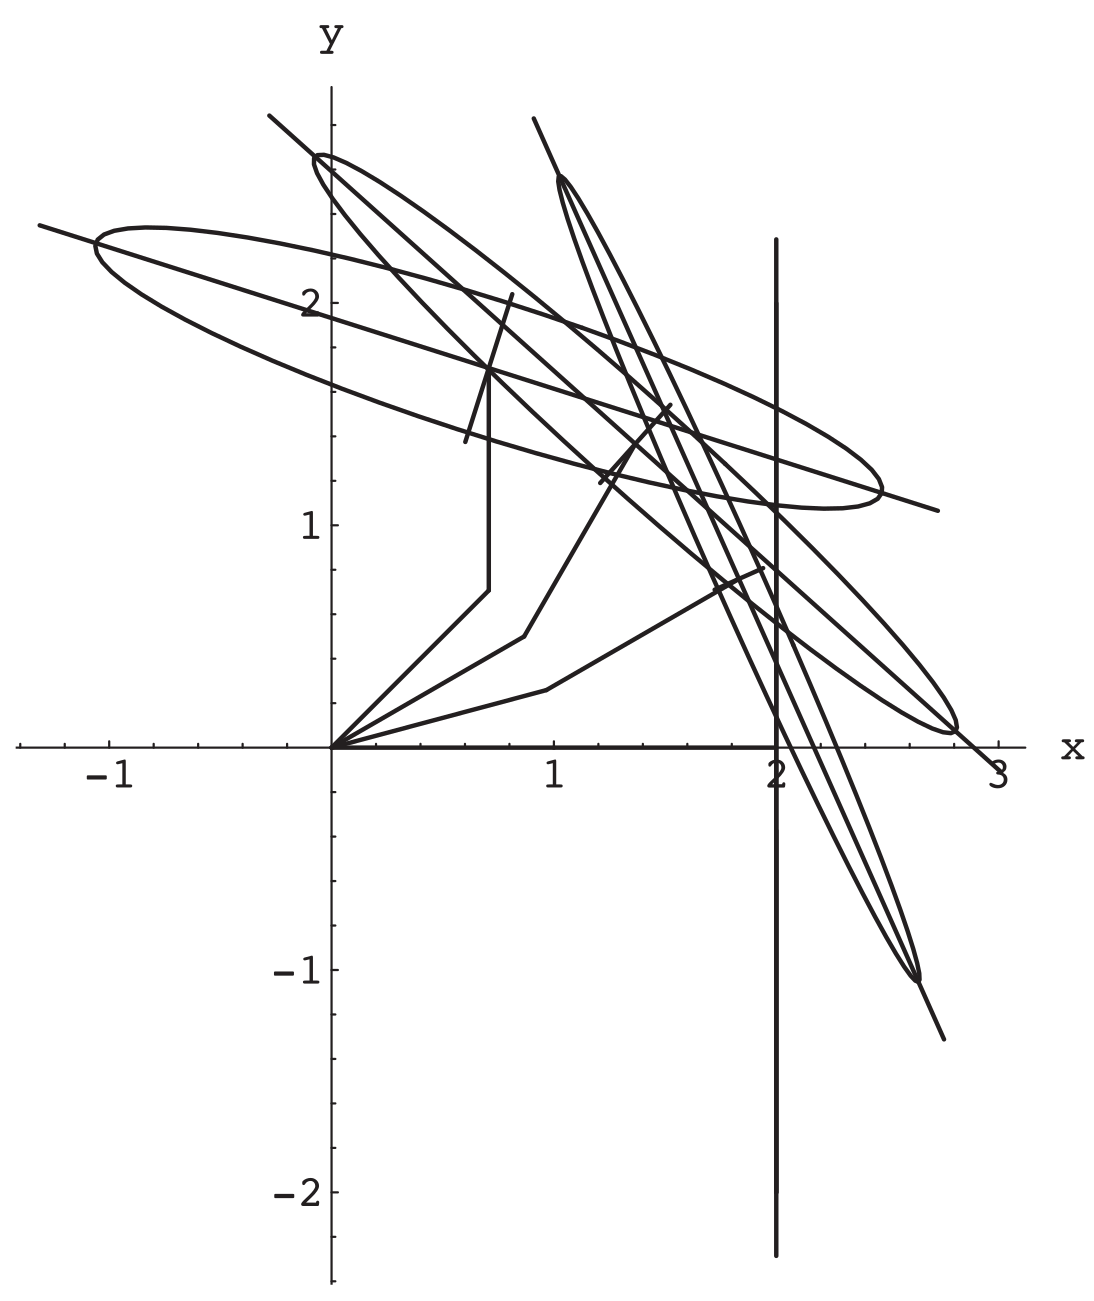
\includegraphics[width=0.85\textwidth]{figures/manipulability_ellipsoids_two_link.png} 
                % \caption{\footnotesize }
            \end{figure}
            \vspace{-2mm}
            \centering
            \footnotesize{Singularity of elbow manipulator with no offsets.}

            \vspace{3mm}
            \only<3>{
            \begin{itemize}
                \item Choose them such that the manipulability $\mu$ is maximized: $a_1 = a_2$.
            \end{itemize}
            }
        \end{column}
    \end{columns}
\end{frame}


\endgroup